\documentclass[article, nojss]{jss}
%%%%%%%%%%%%%%%%%%%%%%%%%%%%%%
%% declarations for jss.cls %%
%%%%%%%%%%%%%%%%%%%%%%%%%%%%%%
%\VignetteIndexEntry{profdpm}
%% almost as usual

\author{Matthew S. Shotwell\\Vanderbilt University}
\title{\pkg{profdpm}: An \proglang{R} Package for MAP Estimation in a Class of Conjugate Product Partition Models}

%% for pretty printing and a nice hypersummary also set:
\Plainauthor{Matthew S. Shotwell} %% comma-separated
\Plaintitle{profdpm: An R Package for MAP Estimation in a Class of Conjugate Product Partition Models} %% without formatting
\Shorttitle{\pkg{profdpm}: MAP Estimation in a Class of Conjugate PPMs} %% a short title (if necessary)

%% an abstract and keywords
\Abstract{
The \pkg{profdpm} package facilitates inference at the posterior mode for a class of product partition models (PPM). Dirichlet process mixtures are currently the only available class members. The PPM is implemented for linear models and multivariate binary models. Several methods are implemented to search for the maximum posterior estimate of the data partition. This article discusses the relevant theory, the \proglang{R} and underlying \proglang{C} implementation, and examples of high level functionality.
}
\Keywords{product partition model, MAP estimate, clustering, \proglang{R}, \proglang{C}}
\Plainkeywords{product partition model, MAP estimate, clustering, R, C} %% without formatting
%% at least one keyword must be supplied

%% publication information
%% NOTE: Typically, this can be left commented and will be filled out by the technical editor
%% \Volume{13}
%% \Issue{9}
%% \Month{September}
%% \Year{2004}
%% \Submitdate{2004-09-29}
%% \Acceptdate{2004-09-29}

%% The address of (at least) one author should be given
%% in the following format:
\Address{
  Matthew S. Shotwell\\
  Assistant Professor \\
  Department of Biostatistics\\
  Vanderbilt University\\
  1161 $21^{\mathrm{st}}$ Ave. South, Nashville, TN\\
  E-mail: \email{matt.shotwell@Vanderbilt.edu}\\
  URL: \url{http://biostat.mc.vanderbilt.edu/wiki/Main/MattShotwell}
}
%% It is also possible to add a telephone and fax number
%% before the e-mail in the following format:
%% Telephone: +43/1/31336-5053
%% Fax: +43/1/31336-734

%% for those who use Sweave please include the following line (with % symbols):
%% need no \usepackage{Sweave.sty}

%% end of declarations %%%%%%%%%%%%%%%%%%%%%%%%%%%%%%%%%%%%%%%%%%%%%%%
\widowpenalty=10000
\clubpenalty=10000
\usepackage{setspace}
\usepackage{amsbsy}
\usepackage{algorithmic}
\newcommand{\bz}{\boldsymbol{z}}
\newcommand{\bu}{\boldsymbol{u}}
\newcommand{\btheta}{\boldsymbol{\theta}}
\newcommand{\bmu}{\boldsymbol{\mu}}
\newcommand{\bphi}{\boldsymbol{\phi}}
\newcommand{\bPhi}{\boldsymbol{\Phi}}
\newcommand{\bbeta}{\boldsymbol{\beta}}
\newcommand{\bgamma}{\boldsymbol{\gamma}}
\newcommand{\bXp}{\boldsymbol{X}^{\prime}}
\newcommand{\bx}{\boldsymbol{x}}
\newcommand{\bX}{\boldsymbol{X}}
\newcommand{\bI}{\boldsymbol{I}}
\newcommand{\byp}{\boldsymbol{y}^{\prime}}
\newcommand{\by}{\boldsymbol{y}}
\newcommand{\bv}{\boldsymbol{v}}
\newcommand{\bm}{\boldsymbol{m}}
\newcommand{\bS}{\boldsymbol{S}}

\begin{document}

\section[Intro]{Introduction}
\pkg{profdpm} is an extension package for the \proglang{R} language and environment for statistical computing \citep{R2011}. This package facilitates inference at the posterior mode in a class of conjugate product partition models (PPM) by approximating the maximum {\it a posteriori} data partition. The class of PPMs is motivated by an augmented formulation of the Dirichlet process mixture, which is currently the only available member of this class. The \pkg{profdpm} package consists of two model-fitting functions, \code{profBinary} and \code{profLinear}, their associated summary methods \code{summary.profBinary} and \code{summary.profLinear}, and a function (\code{pci}) that computes several metrics of agreement between two data partitions. The \pkg{profdpm} package was designed to be extensible.

The remainder of this article proceeds as follows: the relevant theory of product partition models is discussed in section \ref{PPMs}, the underlying \proglang{C} methods are detailed in section \ref{Code}, discussion and examples are presented in sections \ref{Examples:profLinear} and \ref{Examples:profBinary}. Section \ref{Extensions} discusses some future directions for the \pkg{profdpm} package.\\

\section[PPMs]{Product partition models} \label{PPMs}
Consider the following hierarchical Bayesian model for a collection of possibly multivariate observations $\by = \{y_1, \ldots, y_n\}$:
\begin{eqnarray}
y_i | z_i = k, \phi_k & \sim & f(y_i|\phi_k) \nonumber \\
\phi_k & \sim & \pi_{\phi}(\phi_k) \nonumber \\
\bz & \sim & \pi_{\bz}(\bz) \propto \prod_{k=1}^r c_k(\bz), \nonumber
\end{eqnarray}
where $\bz = \{z_1, \ldots, z_n\}$ is a collection of cluster membership variables such that $z_i = k$ indicates observation $i$ is a member of cluster $k$. The collection $\bz$ represents a partition of $\by$ into $r$ clusters, identified by the $r$ unique values among $\bz$. The values of $\bz$ are not important, as long as they are distinct. For simplicity, the positive integers are used to enumerate the distinct values. The tilde symbol `$\sim$' is read `independently distributed as'. The function $f$ is a probability density indexed by parameter $\phi_k$. For $k = 1,\ldots,r$, $\phi_k$ are independently distributed according to prior density $\pi_{\phi}$. The prior mass function $\pi_{\bz}$ is proportional to a product of {\it cohesion} functions $c_k$, which specify the prior distribution of the data partition. The Dirichlet process mixture has a PPM representation when $c_k(\bz) = \alpha\Gamma(n_k)$, where $\alpha$ is the scalar Dirichlet process `precision' parameter, $\Gamma$ is the gamma function, and $n_k$ represents the number of observations assigned to the $k^{th}$ cluster. Alternative cohesions yield other well-known process mixtures \citep[for a partial listing, see][]{LauGreen2007}. The posterior distribution over the data partition is proportional to the product
%The \pkg{profdpm} package extends the Dirichlet process mixture cohesion to include a scalar `balance' parameter $\lambda$, such that $c_k(\bz) = \alpha\Gamma(n_k)^{\lambda}$.  The value of $\lambda$ affects the balance of partition cluster sizes $\{n_1, \ldots, n_r\}$.
\begin{eqnarray}
p(\bz|\by) \propto \prod_{k=1}^r c_k(\bz) \int L(\phi_k|\by,\bz) \pi_{\phi}(\phi_k) d\phi_k , \label{eqn:posterior}
\end{eqnarray}
where $L(\phi_k|\by) = \prod_{i=1}^n f(y_i|\phi_k)^{I(z_i=k)}$ is the cluster-specific likelihood. Hence, the product partition model is conjugate in the sense that both prior and posterior may be written as a product of cluster-specific terms. Further details regarding the PPM are given in \citet{Hartigan1990} and \citet{BarryHartigan1992}.

A maximum {\it a posteriori} (MAP) estimate of the data partition variable $\bz$ partitions the data into clusters. The principal difficulty with MAP estimation is the size of the partition space \citep[see the `Bell number',][]{Bell1934, Rota1964}. Hence, computing the MAP estimate using enumerative methods is not practical.


{\it Profile inference} about the parameter $\phi_k$ is conditional on an estimate of the data partition. Conditional on the estimate, $\{\phi_1, \ldots, \phi_r\}$ are independent {\it a posteriori}, and distributed according to 
\begin{displaymath}
p(\phi_k | \by, \hat{\bz}) \propto L(\phi_k|\by, \hat{\bz}) \pi_{\phi}(\phi_k).
\end{displaymath}
For PPMs implemented in the \pkg{profdpm} framework, the likelihood and prior over $\phi_k$ are selected to be conjugate in $\phi_k$. Hence, the integral in expression (\ref{eqn:posterior}) has simplified form.

The \pkg{profdpm} package computes a MAP estimate for two types of PPMs, corresponding to the \proglang{R} functions \code{profLinear} and \code{profBinary}. Both functions accept model formulae, and return an instance of the class \code{profLinear} or \code{profBinary} respectively. Instances of these classes consist of a data partition estimate and other information related to profile inference. 

\subsection{Product partition of linear models}

The \code{profLinear} function fits a product partition of conjugate normal linear models:
\begin{eqnarray}
y_i | \bx_i, z_i = k, \bmu_k, \tau_k & \sim & N(\bx_i^{\prime}\bmu_k, \tau_k) \nonumber \\
\bmu_k, \tau_k & \sim & N_qG(\bm_0, s_0I_q, a_0/2, 2/b_0) \nonumber \\
\bz & \sim & \pi_{\bz}(\bz) \propto \prod_{k=1}^r \alpha \Gamma(n_k),
\end{eqnarray}
where $y_i$ is a continuous scalar observation, $\bx_i$ is a covariate vector of dimension $q$, $N$ represents the normal distribution with mean $\bx^{\prime}\bmu_k$ and precision $\tau_k$, and $N_qG$ represents the $(q+1)$-variate normal-gamma distribution with mean $\bm_0$, precision matrix $\tau s_0I_q$, shape $a_0/2$, and scale $2/b_0$. The observation vector and design matrix are specified using the \proglang{R} formula mechanism. The prior parameters $\bm_0$, $s_0$, $a_0$, $b_0$, and $\alpha$ may also be specified as arguments to \code{profLinear}. Conditional on an estimated partition, the pairs $\{(\bmu_1, \tau_1), \ldots, (\bmu_r, \tau_r)\}$ are independent {\it a posteriori} and distributed according to the $(q+1)$-variate normal gamma distribution with mean $\bm_k$, precision matrix $\tau\bS_k$, shape $a_k/2$, and scale $2/b_k$. The posterior statistics $\bm_k$, $\bS_k$, $a_k$, and $b_k$ are returned by \code{profLinear} for each cluster.

\subsection{Product partition of binary models}

The \code{profBinary} function fits a product partition of conjugate binary models:
\begin{eqnarray}
y_{ij} | z_i = k, \phi_{kj} & \sim & B(\phi_{kj}) \nonumber \\
\phi_{kj} & \sim & \beta(a_0, b_0) \nonumber \\
\bz & \sim & \pi_{\bz}(\bz) \propto \prod_{k=1}^r \alpha \Gamma(n_k),
\end{eqnarray}
where $y_{ij}$ for $j = 1,\ldots,q$ is the $j^{th}$ binary observation for a subject $i$, $B$ represents the Bernoulli distribution with probability $\phi_{kj}$, and $\beta$ represents the beta distribution with shape parameters $a_0$ and $b_0$. Conditional on an estimated partition, $\phi_{kj}$ are independently beta distributed {\it a posteriori} with shape parameters $a_{kj}$ and $b_{kj}$. This PPM models multivariate binary outcomes only ({\it i.e.} without covariates). Hence, the set of outcomes is specified by supplying a one-sided \proglang{R} formula. The \code{profBinary} function returns the posterior statistics $a_{kj}$ and $b_{kj}$ for $k=1,\ldots,r$ and $j=1,\ldots,q$.


\subsection[Estimation]{Partition Estimation} \label{Estimation}
The \pkg{profdpm} package utilizes four methods to approximate the MAP estimate in an iterative fashion. The first method is the agglomerative method of \citet{Ward1963}, later used by \citet{Heard2005} in the context of Dirichlet process mixtures. Initially, all observations are partitioned into separate clusters. Two clusters are merged at each subsequent step such that the change in marginal posterior mass is largest. This process repeats until all observations are partitioned into a single cluster. This method produces a deterministic and finite sequence of data partition estimates. The estimate with largest marginal posterior mass is selected to approximate the MAP estimate. Although the agglomerative method evaluates the marginal posterior mass function $O(n^2)$ times, this method is usually the second fastest among the implemented methods. This method does not yield arbitrarily precise approximations to the MAP estimate, but performs well in practice.

The second method is the Polya urn Gibbs sampler of \citet{MacEachern1994}, \citet{BushMacEachern1996}, and \citet{MacEachernMuller1998}. The Gibbs sampler sequentially samples from the full conditional distributions having mass functions of the form $p(z_i|\bz_{-i},\by)$, where $\bz_{-i}$ is the collection of cluster membership variables with the exception of $z_i$. The Gibbs method produces a sequence of MAP approximations by selecting the sample MAP estimate at each iteration. This sequence yields arbitrarily precise approximations to the MAP estimate, and is guaranteed to find the MAP estimate in finite time. However, the Polya urn Gibbs sampler is prone slow mixing in the partition space, and is computationally intensive.

The third strategy is a variant of the Sequential Update and Greedy Search (SUGS) method proposed by \citet{WangDunson2010}. The SUGS algorithm assigns observations to clusters sequentially. Initially, the first observation forms a singleton cluster. Subsequent observations are assigned to an existing cluster, or form a new singleton cluster by optimizing the associated posterior probability, conditional on previous cluster assignments. The entire process is repeated in random order. That is, over repeated application, the result is independent of the original data ordering. SUGS is the fastest optimization method, but may perform poorly in MAP estimation of data partitions. Indeed, SUGS was designed for nonparametric applications where the data partition is a nuisance parameter. Hence, SUGS is usually reserved for initial partitioning.

The last method is an iterative stochastic search utilizing `explode' and `merge' operations on the clusters of a partition. At the explode step, a randomly selected subset of observations are redistributed uniformly at random to an existing or new cluster. Each of the exploded observations are then merged with one of the existing clusters in a sequentially optimal fashion. The explode-merge method is motivated by the split-merge Metropolis Hastings algorithms of \citet{GreenRichardson2001}, and \citet{JainNeal2004, JainNeal2007}. This method utilizes a Markov chain to approximate the MAP estimate, but does not sample from the posterior distribution over the data partition. Hence, the explode-merge method avoids the complexity and computational expense of ensuring the chain is ergodic. 

The following pseudocode describes the stochastic method at iteration $t$:
{
\singlespacing
\begin{algorithmic}[1]
    \STATE set $\bz^{\prime} = \bz^{(t)}$
    \STATE draw $n_J$ from $\{1,\ldots,n\}$
    \STATE draw vector $J$ of length $n_J$ from $\{1,\ldots,n\}$ w/o replacement
    \FOR{$j$ in $J$}
	\STATE draw $z_j^{\prime}$ from $\{1,\ldots,n\}$ (explode step)
    \ENDFOR
    \IF{$p(\bz^{\prime}|\by) > p(\bz^{(t)}|\by)$}
	\RETURN $\bz^{\prime}$
    \ENDIF
    \FOR{$j$ in $J$}
	\STATE set $z_j^{\prime}$ to maximize $p(z_j^{\prime}|\bz_{-j}^{\prime},\by)$ (merge step)
    \ENDFOR
    \IF{$p(\bz^{\prime}|\by) > p(\bz^{(t)}|\by)$}
	\RETURN $\bz^{\prime}$
    \ELSE
	\RETURN $\bz^{(t)}$
    \ENDIF
\end{algorithmic}
}  
The explode-merge optimization terminates when the change in $p(\bz^{\prime}|\by)$ from one iteration to the next is less than a threshold value ({\it i.e.} the \code{crit} argument to \code{profBinary} and \code{profLinear}). Because the partition state is discrete, improvements in the marginal posterior mass may be irregular. The \pkg{profdpm} package implements a moving-average in calculating improvement.

\section[Code]{Programming strategy} \label{Code}

The \pkg{profdpm} package is primarily implemented in \proglang{C} (following the \proglang{C99} standard) to facilitate efficient and flexible usage of memory, enable direct interface with the BLAS and LAPACK matrix libraries, and to ease translation to environments other than \proglang{R}.

Product partition models are implemented as a state machine. The model state is represented using the \proglang{C} \code{struct pdpm\_t}, declared in \code{src/profdpm.h} as follows (edited for this document):
\begin{verbatim}
typedef struct pdpm_t {
unsigned char   flags;
double          alp;     //DP precision parameter
unsigned int    ngr;     //number of groups
unsigned int    ncl;     //number of clusters
unsigned int  * vcl;     //cluster membership array
unsigned int  * gcl;     //number of groups per cluster array
double          logpval; //unnormalized log posterior value

void         (*move)( struct pdpm_t * obj,\
                 unsigned int grp, unsigned int cls );
double       (*logp)( struct pdpm_t * obj );
double       (*logponly)( struct pdpm_t * obj,\
                 unsigned int * only, unsigned int size );

void          * model;   //model specific/private data
} pdpm_t;
\end{verbatim}

The \code{flags} member of \code{struct pdpm\_t} is a bitmask for flags, for example, to indicate that convergence criteria for an optimization strategy are met. The \code{alp} member is the Dirichlet process precision parameter $\alpha$. In the \pkg{profdpm} framework, multivariate observations, or univariate observations that should always be clustered together are called `groups'. When no complex grouping structure is present, each observation forms a singleton group. Clusters consist of one or more groups. The \code{ngr} and \code{ncl} members of \code{struct pdpm\_t} store the number of groups and clusters that comprise the PPM state, respectively. Each group is assigned exactly one cluster, identified by an integer stored in the \code{vcl} array. Hence, \code{vcl[4]} indexes the cluster number for group four. For groups that are not yet assigned to a cluster ({\it i.e.} during initialization), the corresponding \code{vcl} entry may take the value defined by the \proglang{C} preprocessor macro \code{BAD\_CLS}. The \code{gcl} array stores the number of groups assigned to each cluster. For example, \code{gcl[3]} indexes the number of groups assigned to cluster number three. Because each group might form a singleton cluster, \code{vcl} and \code{gcl} are both allocated to have length \code{ngr}. The \code{logpval} member stores the unnormalized log posterior mass value at the current state.

The \pkg{profdpm} package implements four methods for partition estimation (see section \ref{PPMs}). Each utilizes a Markov-like process. That is, a model state is initialized and updated sequentially, where the updated state depends on the previous state. Each of the four methods decompose into a series of just two simple operations on the model state: (1) reassigning a single observation from one cluster to another, and (2) computing the marginal posterior mass at the current partition estimate.

For example, consider the SUGS optimization strategy. At iteration $t$, group $t+1$ is either assigned to an existing cluster, or assigned to a new cluster. In order to evaluate the alternatives, group $t+1$ is reassigned to each potential cluster in sequence. The marginal posterior mass is evaluated after each reassignment. Finally, group $t+1$ is reassigned to the cluster corresponding to the largest in posterior mass. Hence, each iteration of the SUGS algorithm decomposes into a series of reassignments and posterior mass calculations. No other operations on the model state are necessary. 
 
Manipulating the model state with simple operations is strategic. By implementing the simple operations efficiently, estimation algorithms may be written generically, and with emphasis on simplicity. Generic application of the estimation routines requires implementing the two simple operations for each specific PPM type ({\it e.g.} two for product partitions of linear models, and two for multivariate binary models).

The \code{move} and \code{logp} members of \code{struct pdpm\_t} are pointers to \proglang{C} functions that implement the reassignment and posterior mass calculation routines. The \code{move} member should point to a function that takes three arguments; a pointer to the PPM state structure (\code{obj}), a group number (\code{grp}), and a cluster number (\code{cls}). That is, in model state \code{obj}, the group with number \code{grp} is reassigned to the cluster with number \code{cls}. The function pointed-to by \code{move} should not return a value, but should update the \code{ncl}, \code{vcl}, and \code{gcl} members to reflect the reassignment operation. The \code{logp} member should point to a function that takes the PPM state structure as an argument, and returns the unnormalized log posterior mass, evaluated at the current model state. The \code{logp} method may or may not update the \code{logpval} member automatically.

The marginal posterior mass function in conjugate PPMs is a product of cluster specific terms. Hence, moving a single group from one cluster to another affects two terms at most. The posterior mass calculation may be optimized by computing only the terms associated with clusters modified since the previous calculation. This optimization is implemented using an optional third \proglang{C} function pointer; \code{logponly}. The function pointed-to by \code{logponly} should accept three arguments; a pointer to the PPM state structure (\code{obj}), an array of cluster numbers (\code{only}), the array's length (\code{size}), and return the partial log posterior mass associated with the clusters referenced in the \code{only} array. In particular, the returned value need only satisfy that the algebraic difference in the return values of two identical calls to \code{obj->logponly} represents the change in log posterior mass associated with model state changes in the period between calls. For example, the following \proglang{C} code updates the log posterior mass associated with a reassignment operation, where \code{obj} is a pointer to an initialized structure of type \code{struct pdpm\_t}:  

\begin{verbatim}
...
cls_from_to[0] = obj->vcl[grp];
cls_from_to[1] = cls_to;
obj->logpval -= obj->logponly(obj, cls_from_to, 2);
obj->move(obj, grp, cls_to);
obj->logpval += obj->logponly(obj, cls_from_to, 2);
...
\end{verbatim}

For model states with many clusters, updating the log posterior mass in this way is often more efficient than recomputing all cluster-specific terms of the log posterior mass function. Initializing the \code{logponly} pointer is optional. When \code{logponly} is left uninitialized (\code{NULL}), estimation routines utilize the \code{logp} pointer instead.

Finally, the \code{model} pointer may be used to store data related to a specific type of PPM. For example, in a PPM of linear models, \code{model} points to a structure that holds the response vector, design matrix, and additional parameter values. The functions pointed-to by \code{move} and \code{logp} may access the structure pointed-to by \code{model}. As a rule, routines that operate generically on the model state, including the four optimization methods should not dereference the \code{model} pointer. 
 
The structure pointed-to by \code{model} may be simple or complex, depending on the resources of the target platform and the available programming effort. A simple model state might store only the original data arrays and other required parameters. When additional memory is available, intermediate values might be cached for more efficient computations. For example, linear models with covariate vector $\bx_i$ often involve the outer product $\bx_i\bx_i^{\prime}$. A computationally efficient method would compute and store this quantity once, rather than recompute the quantity on demand. Furthermore, since $\bx_i\bx_i^{\prime}$ is symmetric, only the upper or lower triangular portion requires storage. The PPM of linear models implemented in the \pkg{profdpm} package utilizes both optimizations.

The \pkg{profdpm} package leaves the programmer to balance the antagonistic relationship between memory usage and computational efficiency by offering a uniform API to partition estimation methods. The \proglang{C} function with prototype \code{pdpm\_t * pdpm\_init(unsigned int ngr)} is a convenience function that allocates memory (using \code{R\_alloc}), partially initializes, and returns a pointer to an instance of \code{struct pdpm\_t}. The argument \code{ngr} specifies the number of groups that comprise the data. However, the structure returned by \code{pdpm\_init} is not fully initialized. The \code{flags}, \code{alp}, \code{model} and function pointer members (except \code{logponly}) of \code{struct pdpm\_t} must be initialized explicitly. Once fully initialized, a pointer to the model state structure is passed to an optimization routine. For example, the function with prototype \code{void method\_fast(pdpm\_t *)} implements the modified SUGS optimization method. When \code{method\_fast} returns, the structure pointed-to by its argument will have been modified (optimized) according to the SUGS algorithm. An interface between \proglang{R} and new PPMs implemented using the \pkg{profdpm} \proglang{C} API must also be written.

\section[Illustration]{Illustration: \code{profLinear}} \label{Examples:profLinear}

The \pkg{profdpm} package adheres to the principle of `convention over configuration'. That is, reasonable default values are selected for model and optimization parameters, but these may also be configured. This strategy may be contrasted with that of the BUGS \citep{LunnSpiegelhalterThomasBest2009} language, where most modeling and sampling aspects must be configured explicitly.   

\subsection[Defaults]{Default Parameters}

By default, the \code{profLinear} and \code{profBinary} functions utilize the agglomerative optimization method. This method is deterministic, relatively fast, and yields MAP estimates that are comparable with other optimization strategies. However, the best MAP approximations are usually obtained using the Gibbs and stochastic search methods, at the expense of additional computation and other consequences of stochastic optimization ({\it e.g.} estimates may not be identical over repeated optimizations). The SUGS method is recommended only for fast initial partition estimation, or in nonparametric applications of the kind considered by \citep{WangDunson2010}.    

All PPMs implemented in the \pkg{profdpm} framework must specify the Dirichlet process precision parameter $\alpha$, which affects the prior distribution over the data partition parameter. Smaller values result in more concentrated prior mass on partitions with fewer clusters. Conversely, larger values for $\alpha$ concentrate prior mass on partitions with additional clusters. This effect may be summarized by computing the prior expected number of clusters. \citet{Antoniak1974} gives two expressions, one approximate and one exact, for the expected number of clusters in a Dirichlet process mixture. The exact expression is given by \[\sum_{i = 1}^n \frac{\alpha}{\alpha + i - 1}.\] The approximate expression is \[\alpha \log\left(\frac{n + \alpha}{\alpha}\right).\] When $\alpha >> 1$, the approximate expression performs well, otherwise the exact expression should be used.

PPMs are often used to detect outlying heterogeneity in otherwise homogeneous observations. The corresponding prior belief dictates that prior mass on the space of data partitions should be concentrated on the partition consisting of just one cluster. For the Dirichlet process mixture, this is enforced by selecting $\alpha$ to be small. The \code{profLinear} and \code{profBinary} functions both set \code{alpha = 1/150} by default. Hence, for $n < 1000$ and $\alpha = 1/150$, the expected number of clusters {\it a priori} is less than $1.05$. Considering that $1.00$ is the minimum expected number of clusters for all $\alpha$ and $n$, taking $\alpha = 1/150$ clearly concentrates prior mass on partitions with few clusters.

The PPM of linear models has four additional prior parameters; $a_0$, $b_0$, $s_0$, and $\bm_0$. Because the model is selected to be conjugate, the posterior parameters may be written in simple terms:
\begin{eqnarray}
\bS_k & = & s_0 \bI_{q} + \bX^{(k)\prime} \bX^{(k)} \nonumber \\
\bm_k & = & \bS_k^{-1}(s_0 \bm_0 + \bX^{(k)\prime} \by^{(k)}) \nonumber \\
a_k  & = & a_0 + n_k \nonumber \\
b_k  & = & b_0 + \by^{(k)\prime}\by^{(k)} + s_0\bm_0^{\prime}\bm_0 - \bm_k^{\prime}\bS_k\bm_k, \label{posterior_stats}
\end{eqnarray}
for $i=1\ldots n$, where $\by^{(k)}$ is the vector formed by concatenating all of the $y_{i}$ in the $k^{th}$ cluster, $\bX^{(k)}$ is the matrix formed by joining as rows, the $\bx_{i}$ of the $k^{th}$ cluster, and $n_k$ is the number of groups comprising the $k^{th}$ cluster.

Equation block \ref{posterior_stats} isolates the influence of prior parameters on posterior quantities. In particular, prior influence may be reduced by setting each parameter close to zero. Note that the prior (normal-gamma) distribution is improper for $a_0$ less than one. However, the posterior is always proper for $n \geq 1$. The \code{profLinear} function specifies $a_0 = 0.001$, $b_0 = 0.001$, $s_0 = 1.000$, and $\bm_0 = [0.000,\ldots,0.000]$ by default. These default values encode a heavy-tailed prior distribution over the linear coefficients, and weights the posterior distribution more heavily by the observed data. 

\subsection[Example]{\code{profLinear} Example}

The following example simulates a dataset consisting of $99$ longitudinal measures on $33$ units of observation, or subjects. Each subject is measured at three times, drawn uniformly and independently from the unit interval. Each measure is drawn independently from the normal distribution with one of three linear mean functions of time, and with unit variance. The linear mean functions each have zero intercept and vary by slope. The longitudinal structure imposes a grouping among measurements on a single subject. Observations grouped in this way should always clustered together. Grouping structure is specified using the \code{group} parameter; a factor that behaves similarly to the \code{groups} parameter of \pkg{lattice} graphics functions. For the PPM of conjugate binary models, the grouping structure is imposed by the model formula. More specifically, grouped observations correspond to rows of the model matrix, resulting from a call to \code{model.matrix} on the formula passed to \code{profBinary}. Hence, the \code{profBinary} function does not have a \code{group} parameter in its prototype. 

The goal of the following example is to recover the simulated partition and conduct profile inference on the slope parameter of each cluster. The following \proglang{R} code block creates and fits the simulated dataset. To ensure that the figures and statistics presented in this document are more reproducible, the pseudo random number generator seed is fixed. 
\begin{Schunk}
\begin{Sinput}
R> set.seed(42)
R> sim <- function(slope.multiplier = 1) {
R+     x <- as.matrix(runif(99))
R+     s <- slope.multiplier * c(-10, 0, 10)
R+     y <- c(s[1] * x[1:33], s[2] * x[34:66], s[3] * x[67:99]) + 
R+         rnorm(99)
R+     group <- rep(1:33, rep(3, 33))
R+     return(data.frame(x = x, y = y, group = group))
R+ }
R> dat <- sim()
R> library("profdpm")
R> fitL <- profLinear(y ~ 0 + x, group = group, data = dat)
\end{Sinput}
\end{Schunk}
The \code{profLinear} returns an object of class \code{profLinear}. The \code{summary.profLinear} method prints and returns (invisibly) summary information regarding the estimated product partition model, including 95\% credible intervals for the linear coefficients under a Laplace approximation to the profile posterior distribution.

Figure~\ref{fig:sim1} presents the simulated data in a scatterplot. For each cluster identified in the estimated partition, the profile posterior mean slope is represented by a dashed line. Approximate $95\%$ credible limits for the slope are represented by flanking solid lines.

\begin{Schunk}
\begin{Sinput}
R> sfitL <- summary(fitL)
\end{Sinput}
\begin{Soutput}
----------
cluster: 1
groups:  11
obs:     33
  estimate lower95 upper95
x   -9.269 -10.196  -8.343
----------
cluster: 2
groups:  11
obs:     33
  estimate lower95 upper95
x   -0.209  -0.650   0.232
----------
cluster: 3
groups:  11
obs:     33
  estimate lower95 upper95
x    8.374   7.196   9.553
----------
\end{Soutput}
\begin{Sinput}
R> plot(dat$x, dat$y, col = grey(0.9), xlab = "x", ylab = "y")
R> for (grp in unique(dat$group)) {
R+     ind <- which(dat$group == grp)
R+     ord <- order(dat$x[ind])
R+     lines(dat$x[ind][ord], dat$y[ind][ord], col = grey(0.9))
R+ }
R> for (cls in 1:length(sfitL)) {
R+     abline(a = 0, b = sfitL[[cls]]$sum$est[1], col = cls, lty = 2)
R+     abline(a = 0, b = sfitL[[cls]]$sum$low[1], col = cls)
R+     abline(a = 0, b = sfitL[[cls]]$sum$upp[1], col = cls)
R+ }
\end{Sinput}
\end{Schunk}

\begin{figure}[h!]
\begin{center}
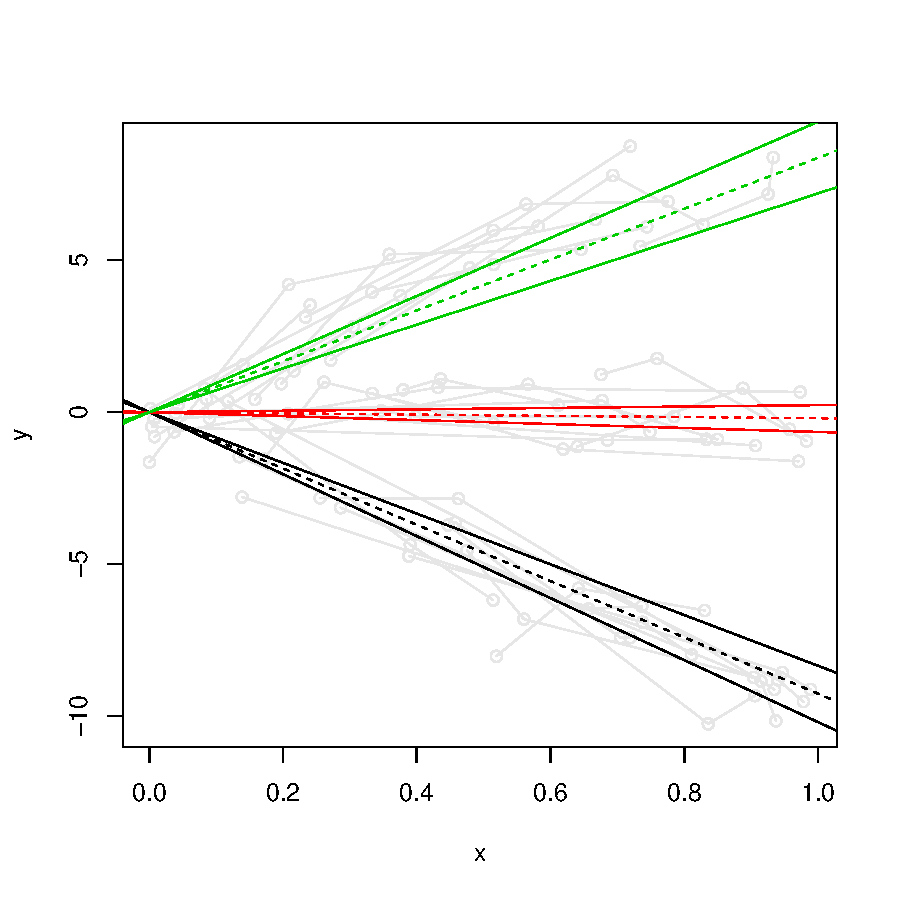
\includegraphics{profdpm-004}
\end{center}
\caption{Scatterplot of three simulated linear subgroups. Mean estimates (dashed) and $95\%$ credible intervals (solid) are presented, conditional on the data partition estimated using the \code{profLinear} function. \label{fig:sim1}}
\end{figure}

\subsection[Comparison]{Partition Comparisons}

Partition estimate comparisons are made using one of many statistics designed for this purpose, including the Rand, Fowlkes and Mallows, Jaccard, and Wallace indices \citep{Rand1971,FowlkesMallows1983,Wallace1983}. Each of these indices assume that a partition is represented by a length $n$ vector of one or more distinct values $\bz = {z_1, z_2, \ldots, z_n}$, where the $z_i$ represents the cluster assignment of observation $i$. Hence, $z_i = z_j$ indicates that observations $i$ and $j$ are assigned to the same cluster. The number of clusters is determined by the number of unique values in the vector $\bz$.

Consider two partitions represented by the cluster assignments $\bz_a$ and $\bz_b$. Let $n_{11}$ be the number of unique ${i,j}$ pairs such that $z_{ai} = z_{aj}$ {\it and} $z_{bi} = z_{bj}$. In words, $n_{11}$ is the count of observation pairs where the pair are clustered together in both partitions. Let $n_{00}$ be the count of observation pairs where the pair are assigned different clusters in both partitions. Hence, $n_{11}$ and $n_{00}$ are the counts of observation pairs where partitions $\bz_a$ and $\bz_b$ are in agreement with regard to cluster assignment. Further define $n_{10}$ as the count of observation pairs where the pair are assigned the same cluster in partition $\bz_a$ but different clusters in partition $\bz_b$, and let $n_{01}$ be the converse. Hence, $n_{01}$ and $n_{10}$ are the counts of observation pairs where partitions $\bz_a$ and $\bz_b$ are discordant. Also observe the equivalence $n(n-1)/2 = n_{11} + n_{00} + n_{10} + n_{01}$, where $n(n-1)/2$ is the number of distinct pairs of $n$ items. Each of the indices mentioned above are a function of these counts.

The Rand index is the most intuitive. It is the proportion of concordant observation pairs: \[\frac{n_{11}+n_{00}}{n_{11}+n_{00}+n_{01}+n_{10}}.\] The Fowlkes and Mallows index is given by \[\frac{n_{11}}{\sqrt{(n_{11}+n_{01})(n_{11}+n_{10})}}.\] The Wallace indices are respectively given by \[\frac{n_{11}}{n_{11}+n_{10}} \quad \mathrm{and} \quad \frac{n_{11}}{n_{11}+n_{01}}.\] The Jaccard index is given by \[\frac{n_{11}}{n_{11}+n_{01}+n_{10}}.\] Each of these indices take values in the closed interval $[0,1]$, where larger values indicate greater agreement. Additional details are found in the cited works.

The \code{pci} function computes each of the partition comparison indices. The returned value is a named vector, where the names indicate the index computed. The Rand, Fowlkes and Mallows, Wallace, and Jaccard indices are abbreviated by \code{R}, \code{FM}, \code{W10}, \code{W01}, and \code{J} respectively. The following demonstrates the \code{pci} function using the estimated and simulated partitions of the previous example.
\begin{Schunk}
\begin{Sinput}
R> simulatedPartL <- rep(1:3, rep(33, 3))
R> estimatedPartL <- fitL$clust
R> pci(simulatedPartL, estimatedPartL)
\end{Sinput}
\begin{Soutput}
  R  FM W10 W01   J 
  1   1   1   1   1 
\end{Soutput}
\end{Schunk}

The estimated partition has good agreement with the simulated partition in the example above, partly due to the large differences in slopes of the simulated linear mean functions relative to the error variance. The grouping structure among longitudinal observations reduces the partition space complexity, further promoting recovery of the simulated partition. 

\subsection[Sensitivity]{Sensitivity to Cluster Homogeneity}

The next example assesses the sensitivity of simulated partition recovery to reduced heterogeneity in the slopes of simulated mean functions. The three slopes in the last example were $-10$, $0$, and $10$. Hence, slope heterogeneity is reduced by multiplying each slope by a proportion. The following \proglang{R} code evaluates the Rand index between the estimated and simulated partition in a series of simulated datasets with reduced slope heterogeneity.

\begin{Schunk}
\begin{Sinput}
R> mult <- rep(seq(1, 0.01, length.out=33), 10)
R> Rand <- sapply(mult, function(mult) {
R+     dat <- sim(mult)
R+     fit <- profLinear(y ~ 0 + x, group=group, data=dat)
R+     pci(rep(1:3, rep(33,3)), fit$clust)['R']
R+ })
R> lws <- lowess(x=mult,y=Rand)
R> plot(lws$x, lws$y, type='l',
R+      xlab='slope multiplier', ylab='Rand index')
R> points(mult + rnorm(length(mult),0,1/200),
R+      Rand + rnorm(length(Rand),0,1/200), col=grey(0.9))
\end{Sinput}
\end{Schunk}

Figure \ref{fig:sim2} illustrates the effect of reduced slope heterogeneity on the Rand index between estimated and simulated partitions. Clearly, there is less agreement in datasets where slope heterogeneity is reduced. Limited or absent grouping information may also hinder recovery of the simulated partition. 

\begin{figure}[h!]
\begin{center}
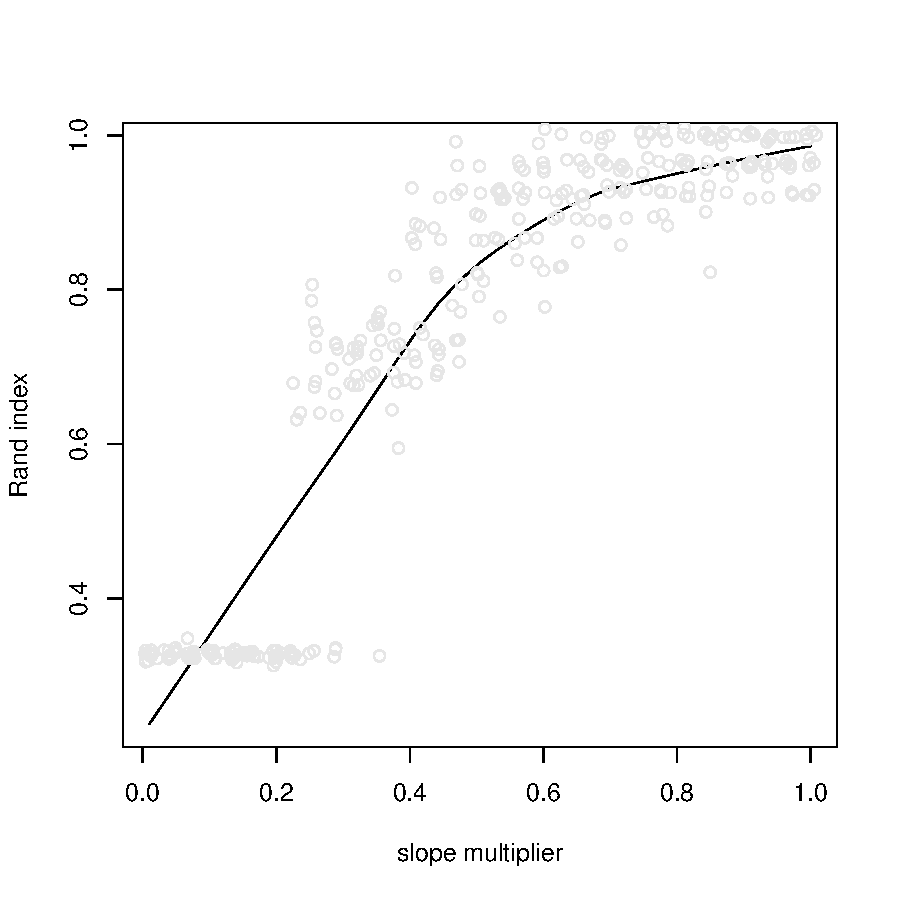
\includegraphics{profdpm-007}
\end{center}
\caption{Scatterplot of Rand indices (between estimated and simulated partitions) versus slope multiplier. Smaller slope multipliers reduce the heterogeneity among simulated clusters. Light gray points represent simulated datasets. Jitter was added to aid in visual discrimination. The black line is a LOWESS estimate of the trend in Rand index versus slope multiplier. For $\alpha$ less than 0.3, the partition estimates mostly consisted on a single cluster. \label{fig:sim2}}
\end{figure}

\vspace{1cm}
\section[Illustrations]{Illustration: \code{profBinary}} \label{Examples:profBinary}

\subsection[Defaults]{Default Parameters}
The PPM of multivariate binary models specifies two prior shape parameters, $a_0$ and $b_0$. For each cluster $k = 1, \ldots, r$ and binary outcome $j = 1, \ldots, q$, the associated posterior probability $\phi_{jk}$ has a beta distribution with shape parameters $a_{kj}$ and $b_{kj}$, given by
\begin{eqnarray}
a_{kj} &=& a_0 + n_{kj} \nonumber \\
b_{kj} &=& b_0 + n_k - n_{kj},
\end{eqnarray} 
where $n_k$ is the number of observations assigned to the $k^{th}$ cluster, and $n_{kj}$ is the number of observations for which $z_i = k$ and $y_{ij} = 1$. That is, $n_{kj}$ is the count of observations in the $k^{th}$ cluster that exhibit outcome $j$. Relative to the data likelihood, the prior influence on the posterior distribution may be reduced by setting $a_0$ and $b_0$ near to zero. Indeed, when $a_0$ and $b_0$ equal zero, the posterior expected probability of outcome $j$ in cluster $k$ is just the associated sample proportion. By default, the \code{profBinary} function takes $a_0$ and $b_0$ to be $1.00$, which encodes a uniform prior distribution over $\phi_{jk}$.

\subsection[Example]{\code{profBinary} Example}
The following \proglang{R} code block simulates a multiple binary outcome dataset with two latent clusters. Each row in the dataset corresponds to a single multivariate binary observation. The \code{profBinary} function automatically clusters observations in a single row. Hence, a \code{group} argument is unnecessary, and not implemented. The outcomes used for partitioning are specified using a one-sided formula.
\begin{Schunk}
\begin{Sinput}
R> p <- seq(0.9,0.1,length.out=9)
R> y1 <- matrix(rbinom(999, 1, p), 111, 9, TRUE)
R> y2 <- matrix(rbinom(999, 1, rev(p)), 111, 9, TRUE)
R> dat <- as.data.frame(rbind(y1, y2))
R> fitb <- profBinary(~0+., data=dat)
\end{Sinput}
\end{Schunk}

Conditional on the estimated partition, the outcome probabilities for each cluster are independently beta distributed {\it a posteriori}. The parameters of the profile posterior distribution for each cluster may be accessed in the return value of \code{profBinary}. In a fashion similar to \code{summary.profLinear}, the \code{summary.profBinary} method computes and prints the profile posterior means and 95\% credible limits of the outcome probabilities for each cluster.

\subsection[Sensitivity]{Sensitivity to DPM Precision $\alpha$}

The value of the DPM precision parameter $\alpha$ has a significant effect on simulated partition recovery in the last example. To illustrate, consider repeating the preceding analysis under a sequence of values for $\alpha$. Figure \ref{fig:sim3} presents the Rand index for the sequence of estimated partitions versus the simulated partition versus $\alpha$.


\begin{Schunk}
\begin{Sinput}
R> alpha <- 10^(-seq(0, 40, length.out=33))
R> Rand <- sapply(alpha, function(alpha) {
R+     fit <- profBinary(~0+., data=dat, param=list(alpha=alpha))
R+     pci(rep(1:2, rep(111,2)), fit$clust)['R']
R+ })
R> lws <- lowess(x=log(alpha),y=Rand)
R> plot(lws$x, lws$y, type='l',
R+      xlab=expression(paste('log', alpha)),
R+      ylab='Rand index')
R> points(log(alpha), Rand + rnorm(length(Rand),0,1/200),
R+      col=grey(0.9))
\end{Sinput}
\end{Schunk}

\begin{figure}[h!]
\begin{center}
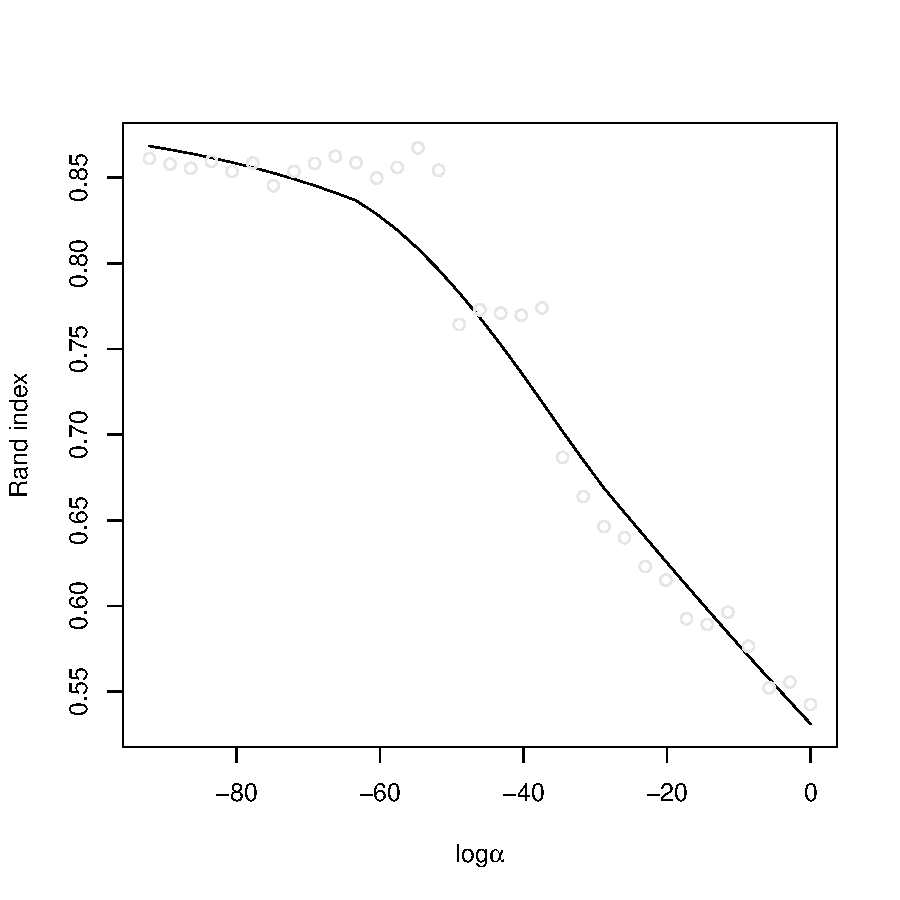
\includegraphics{profdpm-010}
\end{center}
\caption{Scatterplot of Rand indices (estimated versus simulated partition) against DPM precision parameter $\alpha$. Smaller $\alpha$ imposes a stronger penalty against partitions with many clusters. Light gray points represent estimated partitions. Jitter was added to aid in visual discrimination. The black line is a LOWESS estimate of the trend in Rand index versus $\alpha$. \label{fig:sim3}}
\end{figure}

In these data, very small $\alpha$ is required to most closely recover the simulated partition. However, in practice, this optimal precision parameter is unknown. To overcome this, we recommend that $\alpha$ be fixed in some principled manner. The default value for $\alpha$ ($1/150$) concentrates prior mass on partitions with few clusters. Even so, the corresponding partition estimate consisted of sixteen clusters in these data, fourteen more than the simulated partition.

\citet{EscobarWest1995} warn that `sensitivity to $\alpha$ is marked', that the Dirichlet process precision is `a critical smoothing parameter', and that the observed data might be used to draw inferences about $\alpha$. The precision parameter is then treated as an unknown parameter with heavily right skewed gamma prior density. Through inspection of the posterior density, the authors conclude that the data are informative about $\alpha$. Posterior inference about $\alpha$ has been adopted in much of the subsequent Dirichlet process literature \citep{BleiJordan2006,DunsonXueCarin2008,RodriguezDunsonGelfand2009,WangDunson2010}.

Since the DP precision is an important smoothing parameter, we are concerned that allowing the data to inform our belief about $\alpha$ may result in too little smoothing. Hence, we recommend fixing $\alpha$. Arguments and experiments regarding fixed precision are also prevalent in the DP literature \citep{BushMacEachern1996, Daume2007, DunsonPark2008}. 

\section[Extensions]{Extensions} \label{Extensions}
The \pkg{profdpm} package is currently limited to product partitions of linear and binary models, and the optimization strategies described above. Additional models may be implemented as need arises. Also, in the current framework, each cluster of the partitioned data is required to have an identical parametric model, albeit with different parameters. This contrasts, for example, with the finite mixture clustering methods implemented in the \pkg{flexmix} package, which allow multiple parametric forms. This type of functionality is possible in the \pkg{profdpm} framework by specifying a sufficiently complex \code{model} structure, and corresponding \code{move} and \code{logp} methods. 

Estimating a partition is computationally intensive, and an open field of computational research. Other aspects of partition estimation are also under scrutiny. For example, recent work by \citet{WangDunson2010} suggest that marginal likelihood optimization may overfit the observed data, yielding more clusters than necessary. The authors recommend a pseudo marginal likelihood (PML) approach, which imposes a leave-one-out cross-validation strategy to penalize extraneous clusters in partition estimates. The \pkg{profdpm} framework has potential to accommodate alternative likelihoods by implementing alternative \code{logp} methods.

Finally, there are plans to extend the \pkg{profdpm} framework to accommodate novel PPMs by modifying the cohesion function in the prior distribution over data partitions (see section \ref{PPMs}). Note that such modifications result in PPMs other than the augmented Dirichlet process mixture. 

\section*{Acknowledgments}
This research was partly funded by the following National Institutes of Health, National Institute of General Medical Sciences, and National Science Foundation funding projects: NIH 1T32GM074934, NIH R03CA137805, NSF DMS0604666, NIH P20RR017696.

\bibliography{profdpm}
\end{document}
